\section{Simulation Study}
\label{sec:simulations}

\textbf{Topologies.} 
We evaluate our approximation algorithms with simulations over synthetic topologies generated using real portions of the North American electric power grid 
(i.e., IEEE bus systems $14$, $30$, $57$, and $118$) as templates \footnote{\url{http://www.ee.washington.edu/research/pstca/}}. 
The bus system number indicates the number of nodes in the graph (e.g., bus system $57$ has $57$ nodes).
It is standard practice in the literature to only use single IEEE bus systems \cite{Baldwin93,Abur06,Mili90,Xu04}.  
We follow this precedent but do not present these results because they are consistent with the trends found using synthetic topologies.
Instead, we focus on synthetic topologies because, unlike simulations using single IEEE bus systems, we can establish the statistical significance of the performance of our greedy approximations.

Since observability is determined by the connectivity of the graph, we use the {\em degree distribution} of IEEE topologies as the template for generating our synthetic graphs.
A synthetic topology is generated from a given IEEE graph by randomly ``swapping'' edges in the IEEE graph. Specifically, we select a random $v \in V$ and then pick a random $u \in \Gamma(v)$. 
Let $u$ have degree $d_u$.  Next, we select a random $w \notin \Gamma(v)$ with degree $d_w = d_u -1$. % {\footnote {\small Here ``random'' means uniformly at random.}
Finally, we remove edge $(v,u)$ and add $(v,w)$, thereby preserving the node degree distribution.
We continue this swapping procedure until the original graph and generated graph share {\em no edges}, and then return the resulting graph.

\textbf{Evaluation Methods.}
We are interested in evaluating how close our algorithms are to the optimal PMU placement. 
Thus, when computationally possible (for a given $k$) we use brute-force algorithms to iterate over all possible placements of $k$ PMUs in a given graph and select the best PMU placement. 
When the brute-force algorithm is computationally infeasible, we present only the performance of the greedy algorithm.
In what follows, the output of the brute-force algorithm is denoted {\tt optimal}, and when we require cross-validation it is denoted {\tt xvoptimal}.

%We consider performance as a function of the number of PMUs,
%We present three different simulations in Section \ref{subsec:synth}-\ref{subsec:ieee}. 
%In Section \ref{subsec:synth} we consider performance as a function of the number of PMUs, and
%in Section \ref{subsec:zero} we investigate the performance impact of the number of zero-injection nodes in the network.
%These two sections use synthetic graphs. We conclude in Section \ref{subsec:ieee}, where we compare these results to the performance over the actual IEEE graphs.

%\subsection{Simulation 1: Impact of Number of PMUs}
%\label{subsec:synth}

\textbf{Simulation Results.}
We vary the number of PMUs and determine the number of observed nodes in the synthetic graph. 
Each data point is generated as follows. For a given number of PMUs, $k$, we generate a graph, place $k$ PMUs on the graph, and then determine the number of observed nodes. 
We continue this procedure until $[0.9(\overline{x}),1.1(\overline{x})]$ -- where $\overline{x}$ is the mean number of observed nodes using $k$ PMUs -- falls within the $90\%$ confidence interval.

In addition to generating a topology, for each synthetic graph we determined the members of $V_I, V_Z$. These nodes are specified for the original graphs in the IEEE bus system database. Thus, 
we randomly map each node in the IEEE graph to a node in the synthetic graph with the same degree, and then match their membership to either $V_I$ or $V_Z$.

%We present here results for solving \maxinc and \xvalpart using synthetic graphs based on IEEE bus $57$.  
Due to space constraints, we only show plots for solving \maxinc and \xvalpart using synthetic graphs based on IEEE bus $57$.  
The number of nodes observed given $k$, using {\tt greedy} and {\tt optimal}, are shown in Figure \ref{fig:bus57}, and Figure \ref{fig:xvbus57} shows this number 
for {\tt xvgreedy} and {\tt xvoptimal}.  Both plots include the $90\%$ confidence intervals. 
Results for synthetic graphs generated using IEEE bus $14$, $30$, and $118$ yield the same trends.

Our greedy algorithms perform well. On average, {\tt greedy} is within $98.6\%$ of {\tt optimal},
is never below $94\%$ of {\tt optimal}, and in most cases gives the optimal result.
Likewise, {\tt xvgreedy} is never less than $94 \%$ of {\tt xvoptimal} and on average is within $97\%$ of {\tt xvoptimal}. In about about half the cases {\tt xvgreedy} gives the optimal result.
These results suggest that despite the complexity of the problems, a greedy approach can return high-quality results. Note, however, that these statistics do not include performance when
$k$ is large.  It is an open question whether {\tt greedy} and {\tt xvgreedy} would do well for large $k$. 

Surprisingly, when comparing our results with and without the cross-validation requirement, we find that the cross-validation constraints have little effect on the number of observed nodes 
for the same $k$. Our experiments show that on average {\tt xvoptimal} observed only $5\%$ fewer nodes than {\tt optimal}.  Similarly, on average {\tt xvgreedy} observes
 $5.7\%$ fewer nodes than {\tt greedy}. This suggests that the cost of imposing the cross-validation requirement is low, with the clear gain of ensuring PMU correctness across the network.


\begin{figure*}[t]
  \begin{center}
    \subfigure[{\tt greedy} vs {\tt optimal}]{\label{fig:bus57}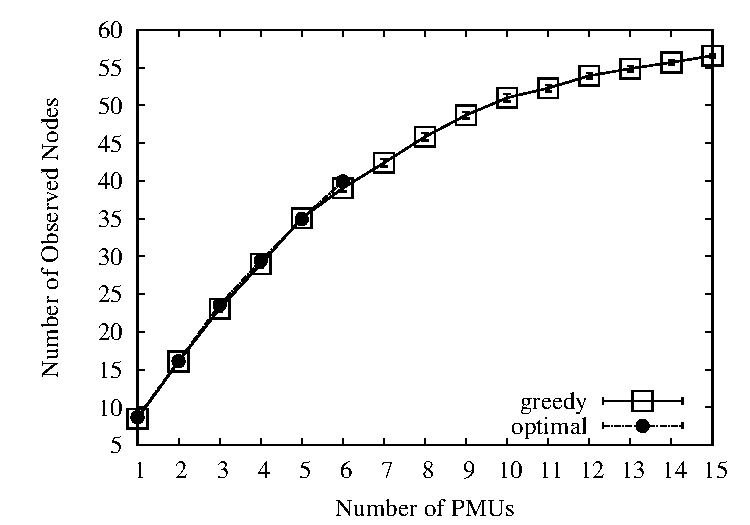
\includegraphics[scale=0.59]{figs/bus57.pdf}}
    \subfigure[{\tt xvgreedy} vs {\tt xvoptimal}]{\label{fig:xvbus57}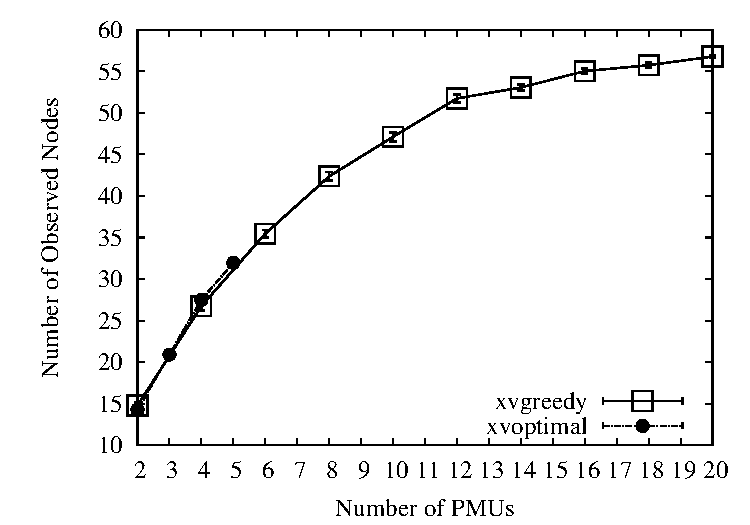
\includegraphics[scale=0.59]{figs/xvbus57.pdf}}
  \end{center}
	\caption{Mean number of observed nodes over synthetic graphs based on IEEE bus $57$ when varying number of PMUs. The $90\%$ confidence interval is shown.}
\end{figure*}






